\documentclass[tikz,border=4pt]{standalone}
\usepackage[T1]{fontenc}
\usepackage{lmodern}
\renewcommand{\familydefault}{\sfdefault}
\usetikzlibrary{shapes.geometric,positioning,arrows.meta,calc,fit,backgrounds,decorations.pathreplacing}
\tikzset{
  node distance=6mm,
  every node/.style={font=\footnotesize,align=center,execute at begin node={\hyphenpenalty=10000\relax}},
  base/.style={draw=gray!60,fill=gray!12,minimum height=7mm,inner sep=2pt},
  term/.style={base,rounded corners=3.5mm,text width=30mm},
  proc/.style={base,text width=32mm},
  err/.style={base,text width=30mm,fill=gray!22},
  io/.style={base,trapezium,trapezium left angle=72,trapezium right angle=108,trapezium stretches=true,text width=28mm},
  dec/.style={base,diamond,aspect=2.4,text width=27mm,inner sep=0pt},
  % predefined process: a call to another procedure
  sub/.style={proc,inner xsep=3mm,path picture={
    \draw[gray!60] ([xshift=1.5mm]path picture bounding box.north west)--([xshift=1.5mm]path picture bounding box.south west)
                   ([xshift=-1.5mm]path picture bounding box.north east)--([xshift=-1.5mm]path picture bounding box.south east);}},
  go/.style={-{Stealth[length=2mm]},draw=gray!55!black},
  lab/.style={font=\scriptsize,fill=white,inner sep=1pt},
  frame/.style={draw=gray!60,dashed,rounded corners=2mm,inner sep=3mm},
  % memory diagrams
  cell/.style={draw=gray!60,fill=gray!12,minimum height=7mm,inner sep=1pt,font=\scriptsize},
  hot/.style={cell,fill=gray!35},
  note/.style={font=\scriptsize,text=gray!30!black},
}

\begin{document}
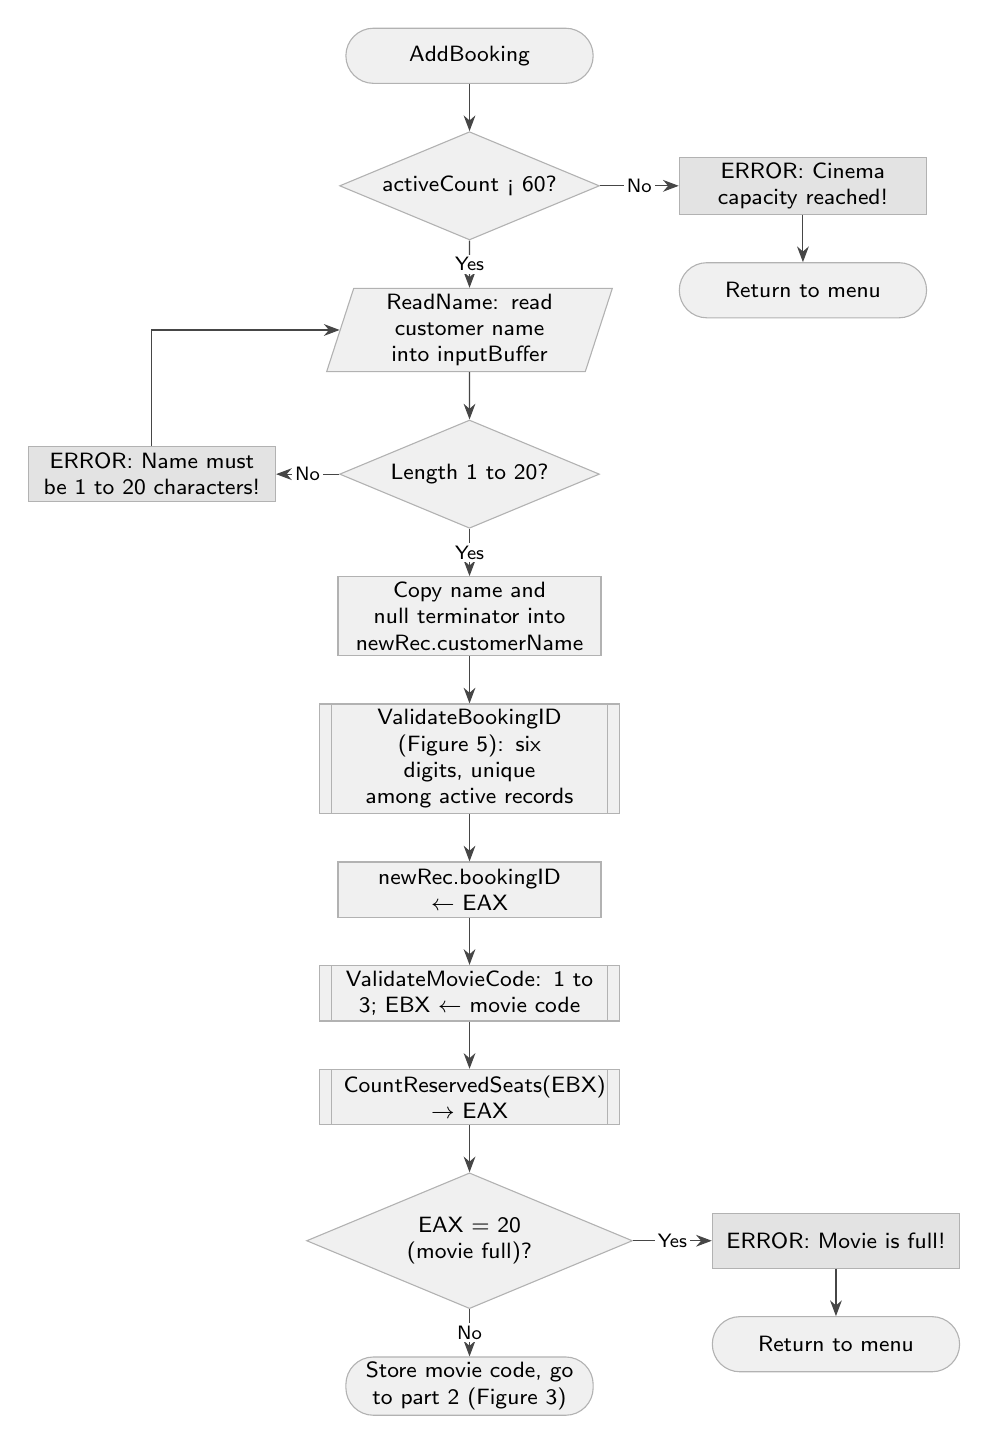
\begin{tikzpicture}
\node[term] (s) {AddBooking};
\node[dec,below=of s] (d1) {activeCount < 60?};
\node[err,right=10mm of d1] (e1) {ERROR: Cinema capacity reached!};
\node[term,below=of e1] (r1) {Return to menu};
\node[io,below=of d1] (n) {ReadName: read customer name into inputBuffer};
\node[dec,below=of n] (d2) {Length 1 to 20?};
\node[err,left=8mm of d2] (e2) {ERROR: Name must be 1 to 20 characters!};
\node[proc,below=of d2] (cn) {Copy name and null terminator into newRec.customerName};
\node[sub,below=of cn] (id) {ValidateBookingID (Figure 5): six digits, unique among active records};
\node[proc,below=of id] (sid) {newRec.bookingID $\leftarrow$ EAX};
\node[sub,below=of sid] (mv) {ValidateMovieCode: 1 to 3; EBX $\leftarrow$ movie code};
\node[sub,below=of mv] (cnt) {CountReservedSeats(EBX) $\rightarrow$ EAX};
\node[dec,below=of cnt] (d3) {EAX = 20 (movie full)?};
\node[err,right=10mm of d3] (e3) {ERROR: Movie is full!};
\node[term,below=of e3] (r3) {Return to menu};
\node[term,below=of d3] (g) {Store movie code, go to part 2 (Figure 3)};
\draw[go] (s)--(d1);
\draw[go] (d1)--node[lab]{No}(e1);
\draw[go] (e1)--(r1);
\draw[go] (d1)--node[lab]{Yes}(n);
\draw[go] (n)--(d2);
\draw[go] (d2)--node[lab]{No}(e2);
\draw[go] (e2.north)|-(n.west);
\draw[go] (d2)--node[lab]{Yes}(cn);
\draw[go] (cn)--(id);
\draw[go] (id)--(sid);
\draw[go] (sid)--(mv);
\draw[go] (mv)--(cnt);
\draw[go] (cnt)--(d3);
\draw[go] (d3)--node[lab]{Yes}(e3);
\draw[go] (e3)--(r3);
\draw[go] (d3)--node[lab]{No}(g);
\end{tikzpicture}
\end{document}
